% Minimal TikZ standalone example
\documentclass[tikz, border=1mm]{standalone}

\usepackage{amsmath,amssymb}
\usepackage{tikz}
\usepackage{tkz-euclide}

\usetikzlibrary{calc,angles,quotes}

\begin{document}
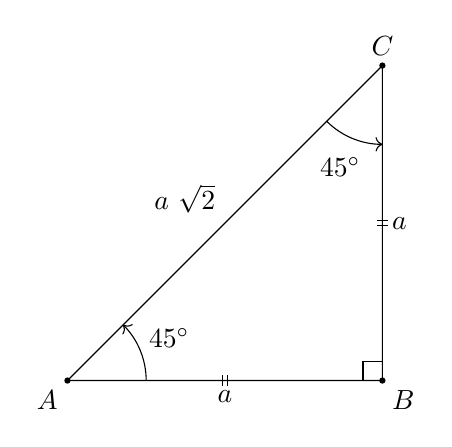
\begin{tikzpicture}[scale=1.0]

	\tikzmath{
		\len = 4.0 ;
	}

	\coordinate (A) at (0,0);
	\coordinate (B) at (\len,0);
	\coordinate (C) at (\len,\len);

	\fill (A) circle (0.4mm);
	\fill (B) circle (0.4mm);
	\fill (C) circle (0.4mm);

	\draw (A) -- (B) -- (C) -- cycle;

	\node[below left] at (A) {$A$};
	\node[below right] at (B) {$B$};
	\node[above] at (C) {$C$};

	\node[below] at ($(A)!0.5!(B)$) {$a$};
	\node[right] at ($(B)!0.5!(C)$) {$a$};
	\node[above left]  at ($(A)!0.5!(C)$) {$a \ \sqrt{2}$};

	\tkzMarkSegments[mark=||, size=2pt](A,B)
	\tkzMarkSegments[mark=||, size=2pt](B,C)

	\pic["$45^\circ$", draw, ->, angle eccentricity=1.4, angle radius=1.0cm]
		{angle = B--A--C};
	\pic["$45^\circ$", draw, ->, angle eccentricity=1.4, angle radius=1.0cm]
		{angle = A--C--B};

	\pic [draw, angle radius=7pt, angle eccentricity=1]
		{right angle = C--B--A};

\end{tikzpicture}
\end{document}
